\section{Black holes in AdS: setup and review}
\label{semiblack}

Just as we did for the 
CFT in its vacuum state, we would now like to re-organize the degrees of
freedom of the CFT, in a heavy typical pure state, into degrees of freedom
that resemble perturbative fields propagating on an AdS black hole
background. 

As we have explained in the introduction, our setup is that we start with
the CFT in a pure state and then allow it to ``settle down'' so that
it resembles a thermal state more and more. When this happens, we 
find that the CFT describes fields propagating in, what is called, the
``eternal AdS black hole.'' 

 Maldacena \cite{Maldacena:2001kr} explained that the eternal AdS black hole has a holographic description in terms of two copies of a CFT in a specific entangled quantum state. In this paper, the eternal black hole geometry will emerge as an auxiliary device for computations done {\it in a single} CFT!

In fact, this is not so surprising from the naive semi-classical perspective since it is indeed true that quantum fields
on a collapsing star start behaving like those in an eternal black hole background, if we probe the
 geometry ``late enough.''  We review these ideas from semi-classical General Relativity in some detail below and we also review the basic formalism of quantizing fields in a black hole background.  The reader who is familiar with
these topics, or is willing to accept our claims, can jump directly to section \ref{sec:outside}.

We wish to emphasize an important logical point. In our construction in sections \ref{sec:outside} and \ref{sec:behind}, we will {\em not assume} any of the claims that we are making in this section. Rather one of the points of our paper is that we independently find a picture in the conformal field theory which is consistent with the
expectations of conventional semi-classical physics. Our review below is meant to (a) remind the reader what these expectations are and (b) serve as a guide --- although not as a logical crutch --- for our later construction. 





\subsection{Collapsing stars and eternal black holes}

In the first part of this section, we review the semi-classical expectation that the details of a collapsing star cease to matter both in front and behind the horizon for ``late enough'' times.
More specifically, and referring to figure \ref{collapseads} 
we have 
\vskip10pt
\noindent {\bf Semi-Classical Expectation:} {\it  Late time bulk correlators in region A and region B of the collapsing star geometry, can be well approximated by correlators in region $\front$ and region $\black$ respectively of the eternal black hole.}
\vskip10pt
\begin{figure}
\begin{center}
\begin{subfigure}[t]{6cm}
\psfrag{Aads}{\rm A}
\psfrag{Bads}{\rm B}
\psfrag{tnot}{$t_0$}
\includegraphics[width=6cm]{collapseads.eps}
\caption{\parbox{5cm}{Collapse of a star (red) to form a black hole in AdS. The matter is injected from the boundary at some time $t_0$. A local observer (black line) dives in much later.} \label{fig:collapsinggeometry}}
\end{subfigure}
\qquad
\qquad
\begin{subfigure}[t]{6cm}
\psfrag{frontads}{$\front$}
\psfrag{backads}{$\other$}
\psfrag{blackads}{$\black$}
\psfrag{whiteads}{\white}
\includegraphics[width=6cm]{kruskalads.eps}
\caption{\parbox{5cm}{AdS eternal black hole , reproduces the measurements of the observer at late times. The quantum fields are placed in the AdS-Hartle-Hawking vacuum.}\label{fig:eternalads}}
\end{subfigure}
\caption{Collapse vs eternal black hole in AdS}
\label{collapseads}
\end{center}
\end{figure}
Here when we say late, we mean late enough so that all the matter has fallen into the black hole and that the fluctuations of the horizon (quasi-normal modes) have mostly decayed away, but not so late that quantum mechanical effects become important. The two timescales have different parametric dependence on $N$ (or $\hbar$) so they can be clearly separated.

For asymptotically flat black holes this claim holds when the eternal black hole is taken in the Unruh vacuum. For black holes formed in AdS --- for instance, by throwing in matter from infinity as in figure \ref{fig:collapsinggeometry} ---, the claim holds when the AdS eternal black hole is taken in the Hartle-Hawking vacuum.\footnote{
The boundary of AdS acts like a reflecting wall, so the radiation coming out of the black hole eventually turns around and falls back in. The Hartle-Hawking state describes an equilibrium configuration where there is no net flux of energy. There is no AdS analogue of the Unruh vacuum.} These results are of course very well known in the context of flat space \cite{Unruh:1976db,birrell1984quantum,Hayden:2007cs} and we believe that they extend naturally
to the case of AdS.






The claim that the geometry outside the black-hole ``settles down'' is probably familiar to most readers; the claim that, at late times, we can replace the entire history of the collapse in region B in figure \ref{fig:collapsinggeometry} by an effective Kruskal geometry is probably less familiar. 
However, the intuitive justification for these statements is the same and can be seen in the Kruskal diagram in figure \ref{fig:kruskal}. 

Within geometric optics, an early-time observer (Observer E) can influence the late-time observer (Observer L) only by emitting a photon or another particle that travels along a trajectory that intersects the world-line of L. However, as L dives in later and later, the window and the solid angle within which E must send his signal becomes smaller and smaller.\footnote{Among other places, this fact was discussed in the works \cite{Susskind:1993mu,Hayden:2007cs,Sekino:2008he} in relation to the consistency between black hole complementarity and the absence of quantum cloning.}

This geometric-optics observation can easily be extrapolated to classical wave mechanics. If we consider a source that emits energy within some solid angle then if we keep the power of the source fixed, its influence at late times diminishes. So, perturbatively, it is clear that a disturbance in the Kruskal geometry at early times cannot influence the late time physics either in front or behind the horizon. The argument that the details of the collapse itself do not matter at late times is an extrapolation from this perturbative argument. 
\begin{figure}
\begin{center}
\psfrag{early}{E}
\psfrag{late}{L}
\includegraphics[width=5cm]{kruskaldiagram.eps}
\caption{Kruskal diagram of AdS eternal black hole. As the observer (L) dives in later, it gets increasingly difficult for any signal from an earlier observer (E) to reach him. }
\label{fig:kruskal}
\end{center}
\end{figure}

Notice that if we fix the time at which the observer L falls in, it is always possible to turn on some matter-excitations which influences the observer. However, these configurations --- while they may be solutions to the equations of motion --- are not relevant as approximations to the geometry of the collapsing black hole.  In our case, as we show in the figure, we create a black hole by turning on a source on the boundary, wait a ``sufficient'' time, and throw the observer L in. By the arguments above, the semi-classical expectation is that this observer should just perceive the geometry of an eternal black hole all along his world line.

One subtle point is that the existence of region $\other$ cannot be neglected in region $\black$. This is because, while classically no influence can propagate from region $\other$ to region $\black$ and influence the late time observer in figure \ref{fig:eternalads}, when we {\em quantize} the field in region $\black$ then, even at late times, it has both ``left-moving modes'' that are analytic continuations of modes from region $\front$ and ``right moving modes'' that are analytic continuations of modes from region $\other$. We return to this in section \ref{modesbrane}.


 



We emphasize again that in our construction, we will not assume either this feature of the quantum mechanics on the eternal AdS spacetime, or the semi-classical general relativity expectation above. Rather we will find both independently in the dual conformal field theory. 



\subsection{Classical Properties of the AdS eternal black hole \label{secadseternal}}

The AdS eternal black hole that we have drawn in figure \ref{fig:eternalads} is a maximal continuation of the AdS-Schwarzschild black hole, just like the Kruskal geometry is a continuation of the Schwarzschild geometry. In this section, we review the metric and geometry of this space in some more detail.
We will  work with the planar version of AdS black holes (i.e. branes). It is straightforward to rewrite everything in terms of AdS black holes with spherical event horizons --- this is even necessary if we wish to address questions related to Poincare recurrence, and other finite volume effects. In this paper, we did not do so since it was more convenient to work with momenta ${\bf k}$ rather than spherical harmonics. 

The metric of the eternal AdS black brane is given by
\begin{equation}
\label{threebrane}
ds^2 = {\ell^2 \over z^2} \left[-h(z) dt^2 + {1 \over h(z)} dz^2 + d\vect{x}^2 \right],
\end{equation}
where \[
h(z) = 1-{z^d \over \zhor^d}.
\]
The horizon is at $z=\zhor$, the boundary at $z=0$ and $\vect{x}$ is a $(d-1)$-dimensional vector. There is no flux turned on here. The metric \eqref{threebrane} is a solution to the equations of motion for the action
\[
S = {-1 \over 16 \pi G_N} \int \sqrt{-g} \left[R + {d(d-1) \over \ell^2} \right].
\]
We have displayed the AdS radius $\ell$ explicitly here because it will make a brief appearance in our discussion of the temperature below.  However, in what follows, and everywhere else,  we will set $\ell = 1$.

We introduce the tortoise coordinate defined by
$
{dz_* \over dz} =- h^{-1}(z)
$. Now the horizon is at $z_*\rightarrow-\infty$. We fix the overall additive ambiguity in the definition of $z_*$ by requiring $z_*\rightarrow 0$ as $z\rightarrow 0$. The metric takes the form
\[
ds^2 = {h(z) \over z^2}(-dt^2 +dz_*^2) +{d\vect{x}^2 \over z^2}
\]
We go to lightcone coordinates
\be
\label{lightconec}
u= t-z_*\qquad,\quad v= t+z_*
\ee
\[
ds^2 = -{h(z)\over z^2} du dv + {d\vect{x}^2 \over z^2}
\]
Here $z$ is defined implicitly via $u,v$ by the previous changes of coordinates. Finally we define
\be
\label{kruskalc}
U = -e^{-{d u \over 2 \zhor}}\qquad,\qquad V = e^{{d v \over 2 \zhor}}
\ee
to get
\begin{equation}
\label{kruskal}
ds^2 = {4 h(z)\over d^2 U V} \left({\zhor \over z}\right)^2
 dU dV +{d\vect{x}^2 \over z^2}
\end{equation}
This metric is originally defined in the region $U<0,V>0$. The future horizon is at $U\rightarrow 0, V={\rm constant}$ and the past horizon at $V\rightarrow 0, U={\rm constant}$. In the form \eqref{kruskal}, it is clear that the metric is smooth at both these horizons and can be smoothly extended past them.\footnote{Near the horizons we have $h \approx {d\over \zhor}(\zhor-z)$. The tortoise coordinate is $z_* \approx {\zhor \over d}\log\left({\zhor-z \over \zhor}\right)$. From the change of coordinates we find $h \approx d e^{d z_* \over \zhor} = d U V.$}
On the other hand there is a specific positive value of $UV$ for which $h$ blows up (in our conventions for $z_*$ this happens at $UV = e^{-\pi}$). These points represent the future and past singularities.


\paragraph{How we take the Large $N$ Limit \\}
Let us pause briefly to specify precisely what we mean by taking the large $N$ limit in the context of this bulk geometry. Although this is a point that seems to cause confusion at times, what we are doing is perfectly conventional. In taking the large $N$ limit, we {\em keep the solution \eqref{threebrane} fixed}. This means that the temperature of the gauge theory also remains fixed and does not scale with $N$. Indeed, the temperature of the black-brane solution \eqref{threebrane} can easily be calculated to be (with all factors restored) 
\[
T = {\hbar c d \over 4 \pi \zhor k_B},
\]
where $c$ is the speed of light and $k_B$ is the Boltzmann constant. Note that $G_N$ does not appear here.  On the other hand, with this fixed temperature, the  ADM mass-density of the black-brane will contain a factor of ${1 \over G_N}$. So the energy density of the boundary CFT does scale with $N$, as we take the large $N$ limit. 

We should point out that $\ell$ also does not appear in the formula for the temperature. This is because we are considering the black-brane solution in AdS. If we were to instead consider the AdS-Schwarzschild solution, then the temperature would depend on $\ell$. Instead of thinking of a black-brane, the reader may instead prefer to think of a {\em big black hole} in AdS i.e. one where the horizon size is larger than the AdS radius.  Such a black-hole is thermodynamically favoured, since the corresponding temperature is higher than the Hawking-Page transition temperature. So, for the conformal field theory on a sphere on radius $R$, our analysis is valid when we take the temperature to be any number larger than the phase transition temperature in units of  ${1 \over R}$, as long as the temperature {\em does not scale with $N$}.  


\subsection{Quantization in an eternal AdS black hole \label{modesbrane}}


We also need to remind the reader how to quantize a field on the background of an eternal AdS black hole. 
In figure \ref{penroseadsb} we see a Cauchy slice for the entire spacetime. 
\begin{figure}
\begin{center}
\psfrag{frontads}{$\front$}
\psfrag{backads}{$\other$}
\psfrag{blackads}{$\black$}
\psfrag{whiteads}{$\white$}
\psfrag{uzero}{U=0}
\psfrag{vzero}{V=0}
\psfrag{s1}{$\Sigma_{\front}$}
\psfrag{s2}{$\Sigma_{\other}$}
\includegraphics[width=10cm]{kruskalads2.eps}
\caption{Cauchy slice for the eternal AdS black brane geometry.}
\label{penroseadsb}
\end{center}
\end{figure}
It can be thought of as the union of two smaller slices, denoted as $\Sigma_{\front}$ and $\Sigma_{\other}$. The slice $\Sigma_{\front}$ is a complete Cauchy slice if we restrict ourselves to events taking place in region $\front$ and the slice $\Sigma_{\other}$ for events in region $\other$. However in order to describe regions $\black$ and $\white$ we need the entire slice $\Sigma_{\front} \oplus \Sigma_{\other}$. When we quantize the field in AdS we impose normalizable boundary conditions at infinity. This means that only the subleading mode (``the vev'') of the field can be turned on. For simplicity we avoid discussing the window of masses where two alternative quantizations are acceptable.

One way to find a complete set of solutions to be used for the quantization, is to first work with the wedge $\front$, whose Cauchy slice is $\Sigma_{\front}$ , and then with the wedge $\other$ and then put them together (the same thing as we do for the quantization of Rindler space or the flat space Schwarzschild solution). So we start with region $\front$.
We consider the black hole solution \eqref{threebrane} and a scalar field obeying
\[
(\Box - m^2) \phi =0 
\]
we consider a solution of the form
\[
f_{\omega,\vect{k}}(t,\vect{x},z) = e^{-i \omega t + i \vect{k} \cdot \vect{x}} \psi_{\omega,\vect{k}}(z)
\]
Plugging into the Klein-Gordon equation we get a second order ordinary differential equation for $\psi_{\omega,\vect{k}}(z)$. 
It has two linearly independent solutions. We impose normalizability of the solution near the boundary i.e.
\[
\psi_{\omega, \vect{k}} (z) \underset{z \rightarrow 0}{\longrightarrow} \normfact^{-1}\,z^{\Delta},
\]
which eliminates one linear combination of the solutions. So, for each choice of $(\omega,\vect{k})$ we have a unique normalizable solution.

We do not impose any boundary conditions at the horizon. Had we imposed ingoing boundary conditions we would have found solutions only for complex $\omega$ i.e. 
the quasinormal frequencies. For the quantization of the field we need to find a complete set of solutions of the wave equation without any restriction on the horizon. 
The solutions that we found are linear combinations of ingoing and outgoing modes. By an appropriate choice of the overall phase, the modes can be taken to be real. 
If we introduce the tortoise radial coordinate $z_*$, in which the horizon is at $z_*\rightarrow - \infty$ we find that the modes behave like
\be
\label{nearhpsi}
\psi_{\omega,\vect{k}}\underset{z \rightarrow z_0}{\longrightarrow} c(\omega,\vect{k})\left(e^{-i\delta_{\omega,\vect{k}}}e^{-i\omega z_*} + e^{i\delta_{\omega,\vect{k}}}e^{i\omega z_*}\right)
\ee
where $c(\omega,\vect{k})$ is a positive real constant.
The relative phase difference $e^{i\delta_{\omega,\vect{k}}}$ is physically meaningful and cannot be removed by changing the conventions.

 
It is also possible to normalize the modes, so that they are canonical
with respect to the Klein-Gordon norm. In this second normalization, we write
\[
\hat{f}_{\omega,\vect{k}}(t,\vect{x},z) = e^{-i \omega t + i \vect{k} \cdot \vect{x}} \hat{\psi}_{\omega,\vect{k}}(z),
\]
where
\[
\begin{split}
&\hat{\psi}_{\omega, \vect{k}} \underset{z \rightarrow z_0}{\longrightarrow} z_0^{d-1 \over 2} \times (e^{-i\delta_{\omega,\vect{k}}}e^{-i\omega z_*} + e^{i\delta_{\omega,\vect{k}}}e^{ i\omega z_* }),\\
&\hat{\psi}_{\omega, \vect{k}} \underset{z \rightarrow 0}{\longrightarrow} c(\omega,\vect{k})^{-1} z_0^{{d-1 \over 2}} z^{\Delta} {1 \over \normfact}.
\end{split}
\]
This notation, where modes that go like ``1'' near the boundary are denoted by  $f_{\omega,\vect{k}}(t,\vect{x},z)$ and those that go like ``1'' near the horizon are denoted by $\hat{f}_{\omega,\vect{k}}(t,\vect{x},z)$ will be used below.

In any case, we have found a complete set of solutions of the Klein-Gordon equation for region $\front$ which can be used to expand the quantum field $\phi$ in region $\front$ in creation and annihilation modes
\[
\phi(t,\vect{x},z) = \int_{\omega>0} {d\omega d^{d-1}\vect{k} \over  (2 \pi)^d}\,\,{1\over \sqrt{2\omega}}\left[a_{\omega,\vect{k}} \hat{f}_{\omega,\vect{k}}(t,\vect{x},z) + \,\,{\rm h.c.}\right]
\]
The modes satisfy the standard commutation relations
\[
[a_{\omega,\vect{k}},a_{\omega',\vect{k}'}^\dagger] = \delta(\omega-\omega')\delta^{d-1}(\vect{k}-\vect{k}')\]
with all other commutators vanishing. 

Notice that the spectrum in $\omega$ is continuous. This does not have to do with the non-compactness of the spatial directions, even if we consider a black hole in global AdS we still 
find a continuous spectrum in $\omega$ --- even though the boundary theory lives on a compact space ${\mathbb S}^{d-1}$. The continuum in $\omega$ is a large $N$ artifact and related
to the approximately continuous spectrum of the dual large $N$ gauge theory in the deconfined phase, see \cite{Festuccia:2005pi, Festuccia:2006sa} for more details.

Following the same analysis in region $\other$ we get another set of creation and annihilation modes that we denote by $\widetilde{a}_{\omega,\vect{k}}$. These modes satisfy an identical-oscillator type algebra among themselves, and commute with all the modes $a_{\omega, \vect{k}}$. If we have the expansion of the field in a complete basis both in regions I and III, it is straightforward to extend it to regions II and IV. 

While it should be obvious from figure \ref{penroseadsb}, we would like to emphasize again that in order to describe a local field in region II (inside the black hole) it is necessary to use {\it both} the operators $a_{\omega,\vect{k}}$ which are visible outside the horizon {\it and} the operators $\widetilde{a}_{\omega,\vect{k}}$ which seem to come from region III. 

Finally let us mention that the natural vacuum for a quantum field in AdS in the presence of a big AdS black hole is the analogue of the Hartle-Hawking vacuum. The Hawking radiation from the black holes
is reflected by the AdS potential and an equilibrium state like that of the flat-space Hartle Hawking state is reached (there is no analogue of the Unruh vacuum). In terms of our oscillators
the Hartle Hawking state is characterized by thermal occupation levels
\be
\label{hhocup}
\langle a_{\omega,\vect{k}} \,a^\dagger_{\omega',\vect{k}'}\rangle_{\rm HH} = {e^{\beta \omega}\over e^{\beta \omega}-1} \delta(\omega-\omega')\delta^{d-1}(\vect{k}-\vect{k}')
\ee
\be
\label{hhocupb}
\langle a_{\omega,\vect{k}}^\dagger \,a_{\omega',\vect{k}'}\rangle_{\rm HH} = {1\over e^{\beta \omega}-1} \delta(\omega-\omega')\delta^{d-1}(\vect{k}-\vect{k}')
\ee
and similar for the modes $\widetilde{a}_{\omega,\vect{k}}$. Here $\beta$ is the Hawking temperature of the black hole \eqref{threebrane}.

%%% Local Variables: 
%%% mode: latex
%%% TeX-master: "infalling_paper"
%%% End: 


